% --------------------------------------------------------------------------
% Template for ICAD-2016 paper; to be used with:
%          icad2016.sty  - ICAD 2016 LaTeX style file, and
%          IEEEbtran.bst - IEEE bibliography style file.
%
% --------------------------------------------------------------------------

\documentclass[a4paper,10pt,oneside]{article}
\usepackage{icad2017,amsmath,epsfig,times,url}
\usepackage{hyperref}
\usepackage{hypcap}
\usepackage{cite}

\usepackage{times}
\usepackage[english]{babel}
\usepackage{flushend}

% Example definitions.
% --------------------
\def\defeqn{\stackrel{\triangle}{=}}
\newcommand{\symvec}[1]{{\mbox{\boldmath $#1$}}}
\newcommand{\symmat}[1]{{\mbox{\boldmath $#1$}}}

\newcommand{\ce}[1]{$\mathrm{#1}$}
\interfootnotelinepenalty=10000
\widowpenalty10000
\clubpenalty10000
% Title.
% --------------------
\title{Illustrating trends in nitrogen oxides \\across the United States using sonification}

% *** IMPORTANT ***
% *** PLEASE LEAVE AUTHOR INFORMATION BLANK UNTIL FINAL CAMERA-READY SUBMISSION *** 

% IF ONE AUTHOR , uncomment this part
%\name{Jyri Huopaniemi} 
%\address{Nokia Research Center \\ 
%Speech and Audio Systems Laboratory \\ 
%P.O.Box 407, FIN-00045 Nokia Group, Finland \\ 
%{\tt jyri.huopaniemi@nokia.com}} 
%

% IF TWO AUTHORS, uncomment this part
\twoauthors{Joshua L. Laughner} {Department of Chemistry \\ University of California, Berkeley \\ Berkeley, CA 94720  USA
\\ {\tt \href{mailto:jlaughner@berkeley.edu}{jlaughner@berkeley.edu}}} {Elliot Kermit Canfield-Dafilou}
{Center for Computer Research \\in Music and Acoustics \\ Stanford University,
Stanford, CA 94305 USA \\ {\tt
\href{mailto:kermit@ccrma.stanford.edu}{kermit@ccrma.stanford.edu}}}


 

%% if necessary, we will uncomment this to reduce the space the bib takes up..
% \let\OLDthebibliography\thebibliography
% \renewcommand\thebibliography[1]{
%   \OLDthebibliography{#1}
%   \setlength{\parskip}{0pt}
%   \setlength{\itemsep}{0pt plus 0.3ex}
% }

\begin{document}
\ninept
\maketitle

\begin{sloppy}

\begin{abstract}
    Leveraging the human auditory system, sonification can be used as an educational tool for non-experts to engage with data in a different mode than visualization.  Without oversimplifying the data, this project presents a sonification tool for exploring \ce{NO_2} and \ce{O_3} data from the BErkeley High Resolution (BEHR) tropospheric \ce{NO_2} and OMO3PR ozone profile datasets.  By allowing the listener control over the data-to-sound mapping and synthesis parameters, one can experience and learn about the interplay between \ce{NO_2} tVCDs and \ce{O_3} concentrations.  Furthermore, interannual trends can be perceived across different types of locations. 
\end{abstract}

\section{Introduction}
\label{sec:intro}

\subsection{Nitrogen oxides play a key role in controlling air quality.}
\label{sec:nox-chemistry}
Nitrogen oxide (\ce{NO}) and nitrogen dioxide (\ce{NO_2}), collectively known as \ce{NO_x}, play an important role in air quality.  Photolysis of \ce{NO_2} produces ozone (\ce{O_3}), and the reaction of \ce{NO} with oxidized volatile organic compounds (VOCs) can lead to the formation of fine particulate matter.

Both ozone and particulate matter concentrations in the atmosphere are regulated by the Environmental Protection Agency (EPA) because of the negative health effects associated with exposure to them. Elevated concentrations of both are known to cause respiratory distress, especially in children \cite{romieu96}. Elevated ozone also damages crops, leading to significant economic losses as well as reducing food yields \cite{tai14}.

The role \ce{NO_x} plays in the production of \ce{O_3} is complex, as the production efficiency of \ce{O_3} depends nonlinearly on both the \ce{NO_x} concentration and the concentrations and identities of VOCs present in the atmosphere. At both high and low concentrations of \ce{NO_x}, \ce{O_3} production due to \ce{NO_x} cycling is suppressed, though for different reasons. At intermediate \ce{NO_x} concentrations, ozone production peaks \cite{murphy07}.  Therefore, cities attempting to improve their air quality by reducing \ce{NO_x} concentrations may see an increase in ozone initially, and a decrease only once \ce{NO_x} concentrations have fallen below a critical point. The value of that critical point depends on the mixture of VOCs present in the atmosphere.

\ce{NO_x} is emitted through a number of anthropogenic and natural processes. Anthropogenic sources are typically those involving combustion, as the high temperatures break the \ce{N_2} and \ce{O_2} molecules in the atmosphere, allowing them to recombine as \ce{NO} or \ce{NO_2}. Examples of such sources are vehicles, power plants, ships, and aircraft. Natural sources include high temperature sources, such as biomass burning or lightning, as well as other sources such as soil bacteria \cite{monks-beirle}.

\begin{figure*}
\centering
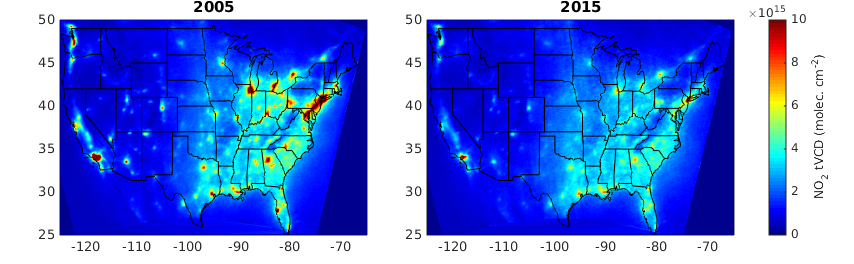
\includegraphics[width=0.9\textwidth]{figs/no2vcds.png} 
\caption{\ce{NO_2} summertime (Apr--Sept) tVCDs from the BEHR product for 2005 and 2015. A clear decrease across the US can be seen.}
\label{fig:sat-obs}
\end{figure*}

\subsection{Space-based measurement of NO$_2$ and O$_3$ offer broad geographic and temporal coverage}

Space-based measurements of \ce{NO_2} tropospheric column density began over two decades ago with the launch of the Global Ozone Monitoring Experiment (GOME) instrument on board the ERS-2 satellite in 1996 \cite{burrows99}. Only \ce{NO_2}, rather than total \ce{NO_x} is measured due to its spectroscopic properties. Since then, several additional instruments have been launched, including the SCanning Imaging Absorption SpectroMeter for Atmospheric CHartographY (SCIAMACHY) \cite{bovensmann99}, Ozone Monitoring Instrument (OMI) \cite{levelt06}, and GOME-2 \cite{callies00}. All these instruments are carried on board polar orbiting satellites which allows them to observe the entire globe in 1--6 days, depending on the instrument and operational mode.

Space-based observations of \ce{NO_2} offer a level of combined spatial and temporal coverage not possible with ground- or aircraft- based instruments.  This offers several notable advantages, such as the ability to observe an entire urban and suburban area, to compare multiple urban areas across the globe using the same instrument, and the ability to monitor episodic events (biomass burning, lightning) difficult to track with other types of instruments.  Multiple papers have made use of these properties to investigate both anthropogenic \cite{ding15, lamsal15, tong15, huang14, vinken14, gu13, miyazaki12, russell12, lin10, kim09} and natural \ce{NO_x} emissions \cite{miyazaki14, beirle10, castellanos14, mebust14, mebust13, zorner16}.

The result of these measurements is a ``tropospheric vertical column density'' (tVCD), usually in units of molecules/cm$^2$. This is the total number of molecules of \ce{NO_2} over one square centimeter of the Earth's surface between the surface and the top of the troposphere (typically $\sim$ 12 km). Rural areas considered ``clean'' typically have tVCDs of $\leq 1 \times 10^{15}$ molec. cm$^{-2}$. Highly polluted areas such as Los Angeles, CA, USA or Beijing, China have tVCDs in excess of $1 \times 10^{16}$ molec. cm$^{-2}$.

Measurements of \ce{O_3} from space can be done similarly to measurements of \ce{NO_2} using ultraviolet-visible spectroscopy and are almost always measured by the same satellites. However, measurements of \emph{tropospheric} \ce{O_3} are complicated by the high concentration of \ce{O_3} in the stratosphere. Whereas the tropospheric and stratospheric components of the total \ce{NO_2} vertical column density are similar orders of magnitude, the tropospheric component of the \ce{O_3} total VCD is minor compared to the stratospheric component \cite{monks-beirle}. Alternatively, the retrieval of tropospheric \ce{O_3} may be done using infrared spectroscopy \cite{nassar08}.

\subsection{NO$_x$ has decreased in the US over the past decade.}
\label{sec:nox-decrease}

In the US, the Environmental Protection Agency (EPA) has regulated measures to decrease the emissions of \ce{NO_x} in order to reduce tropospheric ozone concentrations \cite{epa99}. Regulations targeted both vehicular emissions \cite{epa16} and power plant emissions \cite{epa-cair}.  Satellite observations of \ce{NO_2} \cite{russell12, kim09, lu15} can clearly see the decrease in \ce{NO_2} throughout the US for the time period 2004 onwards (Fig.~\ref{fig:sat-obs}).

\subsection{Sonifcation is an ideal educational tool to communicate the complexity of NO$_x$/O$_3$ chemistry.}

\begin{figure}
\centering
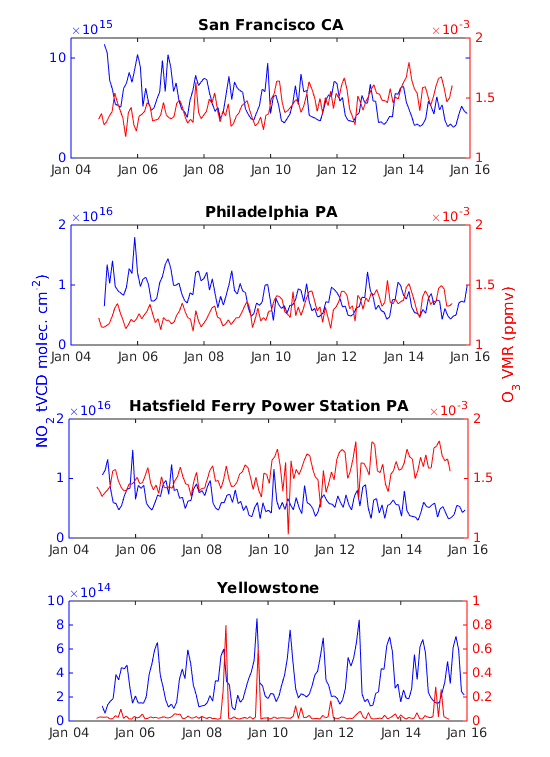
\includegraphics[width=0.95\columnwidth]{figs/four-site-trends.png} 
\caption{\ce{NO_2} tVCD and \ce{O_3} surface concentration trends at two cities (San Francisco, CA and Philadelphia, PA), one coal-fired power plant (Hatsfield, in Masontown, PA) and Yellowstone National Park (WY).}
\label{fig:trends}
\end{figure}

\ce{NO_x} and \ce{O_3} have interesting temporal patterns on both the interannual and seasonal time scales. As discussed in \S\ref{sec:nox-decrease}, \ce{NO_x} has, in general, decreased across the US in the past decade. \ce{NO_x} tVCDs also follow a seasonal cycle, primarily due to temperature dependent shifts in the chemistry. This leads to a sinusoidal pattern superimposed on top of the interannual decrease.  The chemistry described in \S\ref{sec:nox-chemistry} means that \ce{O_3} concentrations will be related to \ce{NO_x} tVCDs, but the exact dependence will vary from location to location.

This is shown in Fig.~\ref{fig:trends} for two cities, one power plant, and one rural area. Both seasonal and interannual trends are clear. The cities and power plants exhibit maximum \ce{NO_2} values in the winter while the rural location does so in the summer. Overall, \ce{NO_2} tVCDs decrease over the cities and power plant while remaining fairly constant over Yellowstone. \ce{O_3} appears to increase over the interannual time scale for the cities and power plant, but not over Yellowstone. 

These characteristics make sonification an ideal way to describe the \ce{NO_x}/\ce{O_3} relationship throughout the US. The temporal dependence of the data lends itself naturally to depiction in a time-dependent medium such as sound. The geographically diverse natural of the dataset can be well represented by the placement of sound in the panning field. By simultaneously representing the \ce{NO_2} tVCDs and \ce{O_3} concentrations at multiple cities, power plants, and rural areas across the US, we provide an intuitive interface for the public to learn about how reductions in \ce{NO_x} concentrations affect \ce{O_3} under different conditions.
	
\begin{figure}[t]
\centering
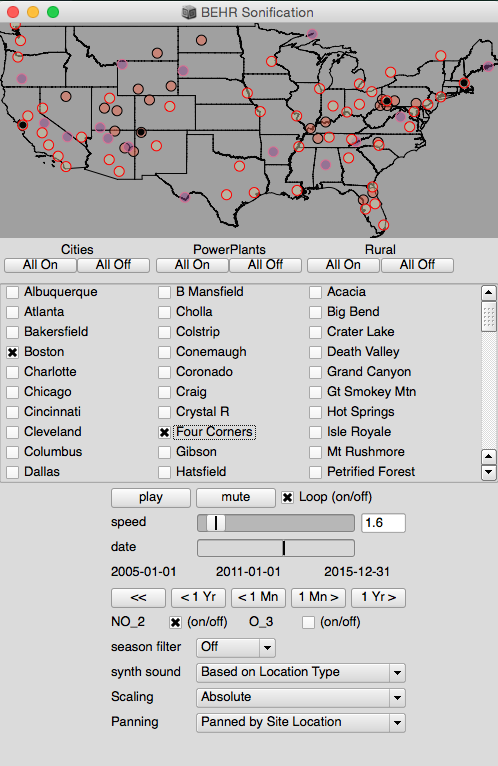
\includegraphics[width=0.95\columnwidth]{figs/gui_revised.png}
\caption{BEHR Sonification GUI.}
\label{fig:gui}
\end{figure}

\section{Approach to sonification}
As an educational tool, sonification allows the user to engage with data through completely different modes than visualization. The streaming capabilities of the human auditory system means that it is good at processing multiple, synchronous data series. As \S \ref{sec:nox-chemistry} describes, the interactions of atmospheric chemicals, meteorological conditions, and ground activity are extremely complicated. Nevertheless, at various time scales, the trends in \ce{NO_2} and \ce{O_3} can be intuitively understood through the auditory experience. Unlike data-music, this sonification project has distinct educational goals and is designed for non-experts in particular. While we strive to reduce the complexity of the data, we want the sonification model to convey useful information.  Furthermore, we want an interface that gives the user flexibility to determine how the data should be presented.  This fulfills the goal to let the user explore the data in a way that conveys pertinent information.  

\subsection{NO$_2$ satellite dataset}
	We make use of v2-1C of the BErkeley High Resolution (BEHR) Ozone Monitoring Instrument (OMI) \ce{NO_2} gridded product, which is publicly available at \url{http://behr.cchem.berkeley.edu/DownloadBEHRData.aspx}. The BEHR dataset is chosen because it uses high-resolution \emph{a priori} \ce{NO_2} profiles that better resolve the urban/rural \ce{NO_2} gradient than the NASA Standard Product or the KNMI DOMINO product. The OMI is carried on board the NASA Aura satellite, launched in 2004, and is a nadir-viewing, UV-visible spectrometer with an overpass time of 13:30--14:00 local standard time \cite{levelt06}.
	
	We use the cities and power plants identified in Russell et al. 2012 \cite{russell12} as the sites for urban and power plant trends. We choose 15 additional sites in rural areas, focusing mostly on national parks, to demonstrate \ce{NO_2} variability in areas substantially less influenced by anthropogenic emissions. The radii for these sites are set to 40 km; this choice is arbitrary, as there is no clear plume to encompass, but is similar to the average radius used for the cities. Monthly average \ce{NO_2} tropospheric vertical column densities (tVCDs) are used to generate the trends. First, the gridded product is restricted to data meeting the following criteria:
	
	\begin{itemize}
	\item Cloud fraction $\leq 0.2$
	\item The XTrackQualityFlags value must be 0 for all pixels that contribute to this grid cell
	\item The vcdQualityFlags must be an even integer (least significant bit is 0)
	\item Only rows 1--58 (0 based indexing) are used due to an issue in v2-1C of the BEHR product that causes the edge rows to be too large.
	% This is NOT the row anomaly; the row anomaly is something very specific with all OMI products
	\end{itemize}
	
	The gridded data is temporally averaged, weighted by the inverse of the pixel areas that contribute to the grid cells. This gives more weight to smaller, more representative pixels.  For each monthly average, the grid cells whose centers are within the radius of the site longitude and latitude given in \cite{russell12} are then themselves averaged to give a single value for each site for each month.

\subsection{O$_3$ satellite dataset}

	We use the OMO3PR ozone profile dataset to obtain tropospheric \ce{O_3} available from \url{https://disc.gsfc.nasa.gov/Aura/data-holdings/OMI/omo3pr_v003.shtml}.   This retrieval uses optimal estimation to fit an \ce{O_3} profile to observed absorbance in two wavelengths. An \emph{a priori} \ce{O_3} profile is used as the basis for the profile shape.  We choose this product because it is also derived from the Ozone Monitoring Instrument, as is our \ce{NO_2} product, and so has similar spatial and temporal coverage. Kroon et al. compared this product against multiple other satellite \ce{O_3} products and \emph{in situ} sonde measurements and found a +30\% bias in the midlatitudes  \cite{kroon11}. While this alone should not interfere significantly in the use of this product for the trend sonification in this work as the bias is systematic, uncertainty in the values will be high due to the challenge of separating tropospheric and stratospheric \ce{O_3}.
	
	A gridded version of this product is not available; therefore we obtain monthly averages differently than with the \ce{NO_2} product. Similarly to \ce{NO_2}, pixels with centers within the radii defined for the geographic sites are identified as contributing to the trend for that site; unlike the \ce{NO_2} product, these are the native satellite pixels, rather than regridded data. All valid pixels for a site for a month are binned in this step. Pixels are considered invalid if:
	
	\begin{itemize}
	\item Cloud fraction for either UV channel is $> 0.2$
	\item Aerosol optical thickness is $> 10^{-5}$. Elevated aerosol layers lead to erroneously large tropospheric \ce{O_3} concentrations \cite{omo3pr-readme}.
	\item The ReflectanceCostFunction field is $> 30$. This indicates erroneous radiance due to the OMI Row Anomaly \cite{row-anomaly}.
	\end{itemize}
	
	For each binned profile, two quantities are calculated. First, the bottom partial column (in Dobson Units) is converted into volume mixing ratio in units of part-per-million by volume (ppmv) using the formula provided in the OMO3PR Readme \cite{omo3pr-readme}. Because this formula relies on the edges of the pressure bin and the lower edge is the surface, we calculate the surface pressure for each profile by interpolating the Global Land One-km Base Elevation (GLOBE) project elevation data \cite{globe} to the pixel latitude and longitude, then convert from altitude to pressure using Eq. \eqref{eqn:pres-scale-height}:
	
	\begin{equation}
	\label{eqn:pres-scale-height}
	p = p_0 e^{-z/H} \,,
	\end{equation}
	where $p_0$ is the sea level pressure of 1013 hPa, $z$ is the altitude in meters, and $H$ is a scale height of 7400 m.
	
	The second quantity is the tropospheric vertical column density (tVCD), which is computed by summing the profile partial columns over all levels with a bottom pressure edge $> 200$ hPa. This is converted from Dobson Units to molec. cm$^{-2}$ by multiplying by $2.69 \times 10^{16}$
molec. cm$^{-2}$ / DU. 

	Both the surface concentrations and tVCDs are averaged over all pixels binned to a given site for a given month. Unlike the \ce{NO_2} product, no weighting for pixel area is applied, as the pixel size is not given in this product.
	 
\subsection{Sonic mappings}
\label{sec:sonic-mappings}
After the preprocessing, we have a set of locations through the United States that each have corresponding time series for \ce{NO_2} tVCDs and \ce{O_3} concentrations. We present several modes for listening to the data. In the simplest case, we use the data for each location as the frequency parameter to a sinusoidal oscillator.  We exponentially map the quantities of the compounds into an audible range according to
\begin{equation}
    c \left[(d/c)^{\frac{x-a}{b-a}}\right]\,,
\end{equation}
where $x$ is the value being mapped from the old range $[a, b]$ to the new range $[c, d]$.  In general, we can constrain \ce{NO_2} and \ce{O_3} to different frequency ranges.  Moreover, we provide three scaling/normalization schemes for mapping the data for each compound at each site to frequency. In order to make comparisons across all sites, we scale the data by the global compound minimum and maximum.  Since this compresses the frequency range of the individual sites, we can also scale the data by each site's individual minimum and maximum. While this makes it impossible to make judgments across sites, it highlights the seasonal and overall trends for individual sites. Last, we can scale the data by the minimum and maximum values of an individual type of location. This is particularly helpful for rural sites, as the quantities of \ce{NO_2} and \ce{O_3} change much less than in cities and power plants. In all cases, as the number of geographical locations increases, it becomes challenging to attend to which time series is which.  

One spatial panning scheme presents each compound on independent speaker channels (e.g., \ce{NO_2} $\rightarrow$ left and \ce{O_3} $\rightarrow$ right).  This  makes it easier to identify the time series related to \ce{NO_2} and \ce{O_3}.  In order to improve the listener's ability to differentiate geographical locations, we also have a second panning scheme that maps each location's longitude and latitude to auditory spatial location. We place the listener in the center of the United States facing north.  We offer a stereo mode, which maps longitude to left and right (i.e. the west coast of the United States to the left and the east coast to the right). An additional quadrophonic mode also maps latitude to front and back; this mode supposes speakers placed directly to the front, back, left, and right of the listener.

Another parameter of the sonification is the sound synthesis. Since Sine waves are challenging to localize in space, it can be hard to differentiate between simultaneously playing sites in the second panning mode. To address this issue, we propose several other sound generators to replace the sine oscillator. These include band-pass filtered noise, sawtooth oscillators, and square oscillators. These can be assigned to each site category; here, we use a square oscillator for cities, a sawtooth oscillator for power plants, and filtered noise for the rural sites. 

One final sonification parameter is a ``season filter'' designed to highlight seasonal fluctuations. This is implemented as a resonant low-pass filter where the cutoff frequency oscillates as a function of season. For each site, the filter cutoff frequency is designed relative to that site's fundamental frequency.  This filters the spectrum and acts as an auditory cue that highlights the effects of seasonal changes. 


% \begin{align}
%     \text{min}_{\text{global}}(\text{\ce{NO_2}}) &\rightarrow
%     \text{min}(\text{freq}_1) \\
%     \text{max}_{\text{global}}(\text{\ce{NO_2}}) &\rightarrow
%     \text{max}(\text{freq}_1) \\
%     \text{min}_{\text{global}}(\text{\ce{O_3}}) &\rightarrow
%     \text{min}(\text{freq}_2) \\
%     \text{max}_{\text{global}}(\text{\ce{O_3}}) &\rightarrow
%     \text{max}(\text{freq}_2)
%     \,,
% \end{align}




\subsection{Sonification interface}

While the synthesis routines do not depend on the GUI, having an interface makes it much easier to understand and control the parameters of the sonification. The GUI, which can be seen in Fig.~\ref{fig:gui}, displays a map of the United State with indicators for where we present data.  These locations are color coded by location type (e.g., power plants, cities, etc.). A bank of check-boxes allow the user to select which locations contribute to the sonification. Naturally, the map is updated to reflect which locations are selected.  


Basic control is provided for playing/pausing and muting/unmuting. We also provide the ability to loop through the data or step through it one month at a time.  Controls are provided to control the speed at which the sonification is performed.  When the data are presented quickly, the listener perceives general trends while at slower speeds the seasonal and monthly trends dominate.  This time resolution control is useful for zooming between micro and macro scales.  

Finally, controls are offered for switching between the various sonification schemes. We provide the appropriate controls to enable/disable features of the model, and when appropriate, control their parameters.  

\section{Evaluation}

To evaluate the effectiveness of the sonification, informal listening tests were performed. Listeners primarily had backgrounds in either atmospheric chemistry or music, but not both. The listening tests involved a pretest to judge each listener's prior knowledge, followed by a guided and unguided exploration of the features and mappings of the sonification to gauge their effectiveness.  We also present our own observations of trends that are evident in the data.

\subsection{NO$_2$ interannual trends}\label{sec:nox-trends-listening}
We found \ce{NO_2} trends are apparent both for a single location and when comparing multiple locations.  When using the global scaling, the seasonal oscillation in \ce{NO_2} tVCDs stands out clearly, especially for cities. For rural environments, the global scaling compresses the values.  This is useful, however, for comparing their absolute levels to urban locations.  Aurally, it is obvious that the overall \ce{NO_2} levels are much lower in rural environments. Using the local scaling, the downward trends and seasonal oscillatory trends become more discernible. 

In general, we found that power plants seem to be less affected by seasonal changes than cities, but listening to the locally scaled version of the power plants makes the seasonal changes more apparent. One interesting observation is that some power plants (e.g., Huntington) start with a sharp decrease in \ce{NO_2} emissions and then level out for the rest of the dataset. Overall, these observations provide compelling evidence for the importance of multiple scaling options.  

We also observe that locations on the East Coast tend to have higher overall levels than elsewhere in the country.  For example, Shenandoah is in rural Virginia, however the \ce{NO_2} levels are comparable to those in Fresno, California.  Naturally, Shenandoah's  \ce{NO_2} levels are influenced by its proximity to large cities like Baltimore. Likewise, trends in Philadelphia and Pittsburgh are highly correlated to one another.

While listening to all sites in a given category simultaneously, listeners were nearly all able to identify that both city and power plant \ce{NO_2} have markedly decreased between 2005 and 2015, while rural \ce{NO_2} remained constant. When asked to identify individual sites with the largest change in \ce{NO_2} tVCDs, listeners were generally able to correctly identify the city with the largest change out of four choices, although this may have been influenced by prior knowledge as very few listeners' confidence in this answer increased after listening. All listeners were able to identify at least one rural site with the largest change out of all fifteen sites, as long as they were permitted to turn individual sites on and off, and about half correctly identified the two rural sites with significantly larger decreases than the other thirteen rural sites. In both cases (comparing four cities and comparing all rural sites), listeners were not able to identify the which site had the largest change when multiple sites were playing simultaneously.  Overall, we succeeded in our basic goal of representing decadal trends in \ce{NO_2} tVCDs.

\subsection{O$_3$ interannual trends}
For evaluation, we use the \ce{O_3} concentrations nearest the surface rather than the partial \ce{O_3} column.  We observe that an overall rise in most cities is readily apparent, as are the seasonal oscillations, even for listeners without extensive knowledge of \ce{NO_x}/\ce{O_3} chemistry.

This indicates that the OMO3PR product shows that \ce{O_3} is increasing on the interannual timescale throughout the US. This is consistent with the hypothesis that \ce{O_3} increases with temperature \cite{lin17}. However, due to the difficulty in retrieving tropospheric \ce{O_3} from space, verifying this with other tropospheric \ce{O_3} satellite products (e.g. \cite{choi08}) should be considered, and comparison to surface-based measurements should be carried out. Additionally, we are planning on including temperature data to demonstrate the relationship between \ce{O_3} and temperature.  Nevertheless, the listener can clearly hear interannual trends in the \ce{O_3} retrieved with the OMO3PR product; thus the sonification itself represents this successfully and can be used with other \ce{O_3} measurements in the future.

Sonifying \ce{O_3} faces some challenges, given that the data has more extreme values compared to \ce{NO_2}. These are comparatively infrequent, but significantly larger than the majority of values.  In our global mapping, this means that the majority of the variability is compressed to a very small range. This can be alleviated by doing the same mapping as described in \S\ref{sec:sonic-mappings}, but by clipping the range to prevent outliers from having such an effect on the rest of the data.  This will make the interannual variability much clearer for most sites, but means the listener cannot compare absolute magnitudes. Given these difficulties and the relatively high uncertainty of the \ce{O_3} product, the informal listening tests did not test the perception of \ce{O_3} trends.
% Additionally, at sites with the infrequent, extreme values (e.g. Los Angeles), hearing the interannual trend even in this ``local'' mode is difficult.

\subsection{Panning, season filter, and synthesis sounds}
In our listening tests, we were particularly interested in the success of these sonic mappings. As predicted by the resolution of human auditory spatial cues, listeners were better able to perceive and interpret longitudinal (left-right) spatial cues than latitudinal (front-back) spatial cues. It is challenging to mitigate this issue outright as we are fighting with a physiological feature of the human auditory system. Perhaps a higher speaker density and a spatially warped panning algorithm would improve the result of the spatial cues. Additionally, the longitudinal panning was insufficient to help most listeners identify individual sites when multiple sites were playing (\S\ref{sec:nox-trends-listening}).  That being said, many listeners remarked that the panning improved their engagement throughout the listening test.  

The season filter was unsuccessful for giving listeners seasonal cues. At high speeds, the cutoff oscillations are pronounced but the data are presented too quickly to make sense of the filtering. At slower speeds, the effects are masked. Both issues are accentuated because, while higher pitches connect very naturally to greater quantities of \ce{NO_2} or \ce{O_3}, the cutoff frequency of a filter has no intrinsic connection to season.  More problematically, some people remarked that the season filter affected their perception of the fundamental pitch used to convey the primary data. As this could confound the primary goal, we want to redesign the implementation of the season filter. One idea is to ``detrend'' the data when the season filter is engaged. By removing the overall (long time scale) trends, the localized fluctuation will hopefully become more pronounced. Another idea would be to allow the user to select which months to hear. Then the listener would not have to rely as much on memory.  For instance, one could listen to only summer months to hear trends in that  annual cycle rather than hearing the full year, or the playback could be set to advance in six-month steps, directly comparing summer and winter months.   

The different sonic oscillators (filtered noise, sawtooth, etc) representing different site types were easy for some listeners to differentiate but challenging for others.  When listening to multiple sites at once, listeners found it more challenging to differentiate between the square and sawtooth waveforms (cities and power plants) than the filtered noise (rural sites). Listeners also found it more challenging to discriminate pitch for the filtered noise.   

\subsection{Relationship between NO$_2$ and O$_3$}

	As described in \S\ref{sec:nox-chemistry}, the changes in \ce{O_3} concentration can be positively or negatively correlated with changes in the \ce{NO_2} tVCDs. The informal listening tests had listeners attempt to identify whether \ce{NO_2} and \ce{O_3} were correlated, anti-correlated, or uncorrelated at Phoenix, AZ. Fig.~\ref{fig:del-del} plots the change in \ce{NO_2} and \ce{O_3} between adjacent data-points as a function of time for Phoenix, AZ. The overall correlation between $\Delta$\ce{NO_2} and $\Delta$\ce{O_3} is negative (where $\Delta$ indicates a month to month difference), although there are times when the correlation is positive. Statistically, there is a very weak negative overall correlation ($R^2 < 0.1)$ between $\Delta$\ce{O_3} and $\Delta$\ce{NO_2} at Phoenix. 
	
	This commingling of positive and negative correlations makes discerning the correlative relationship between $\Delta$\ce{NO_2} and $\Delta$\ce{O_3} sonically difficult. An additional element of difficulty comes from the high uncertainty in the chosen \ce{O_3} satellite product. Future refinements will explore using alternate sources of \ce{O_3} data, including other satellite products and direct surface measurements of \ce{O_3}.
	
	\begin{figure}
	\centering
	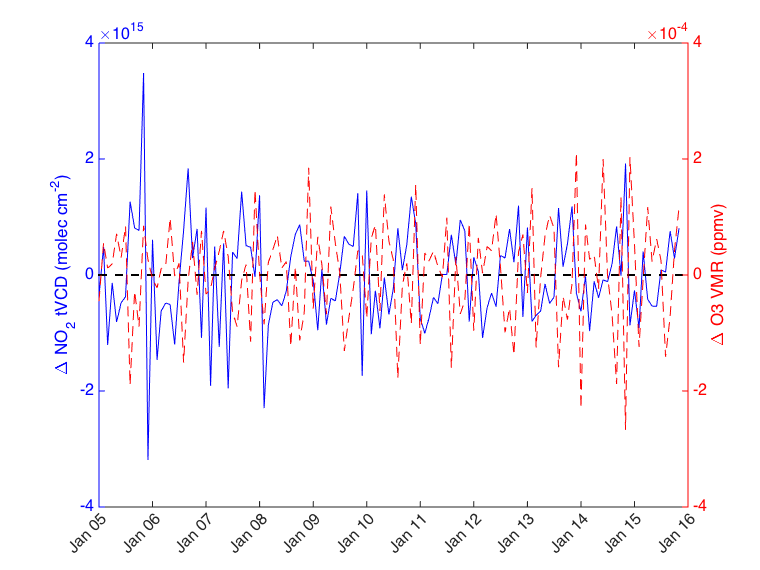
\includegraphics[width=0.95\columnwidth]{figs/delta-delta-timeser-phoenix_AZ.png} 
	\caption{Delta-delta time-series plot of \ce{O_3} and \ce{NO_2} for Phoenix, AZ. Each point is the difference in \ce{NO_2} tVCD or \ce{O_3} concentration between that month and the following month.}
	\label{fig:del-del}
	\end{figure}
	
	For the purpose of evaluating the effectiveness of our sonification at communication the \ce{NO_2}/\ce{O_3} relationship, we judge whether listeners identified the overall correlation: that \ce{NO_2} and \ce{O_3} are negatively correlated at Phoenix, AZ. Most listeners' response after listening moved towards anti-correlated compared to their pretest response. About half of listeners completely reversed their response after listening from correlated to anti-correlated. Therefore, we judge our sonification to be moderately successful at communicating the \ce{NO_2}/\ce{O_3} relationship in this case.

\section{Conclusions}
In this paper, we have described a sonification tool for comparing trends in \ce{NO_2} tVCDs and \ce{O_3} concentrations across the United States.  Overall, informal listening tests have shown that untrained listeners can readily identify interannual trends and identify which sites exhibit the largest changes in \ce{NO_2}.  Clearly, there is more work to be done. We need to provide additional data such as temperature and humidity as well as ground based measurements to improve the educational value of presenting the data as a sonification for untrained listeners.  Certain secondary elements of the sonfication, particularly representing seasonal differences and the geographical position through panning need additional development to make them fully effective.  Furthermore, while this project focuses on an experiential auditory experience for non-experts, we should provide more visual feedback (e.g., generating plots on-the-fly that correspond to the sonification) as an additional avenue for learning about \ce{NO_2} and \ce{O_3} trends.  


\section{ACKNOWLEDGMENT}
\label{sec:ack}

JLL acknowledges support from NASA through the Earth and Space Science Fellowship NNX14AK89H, NASA grants NNX15AE37G and NNX14AH04G, and the TEMPO project grant SV3-83019.  JLL also thanks Ronald C. Cohen for advice and support as a Ph.D. advisor. EKCD's research reported in this publication was partially supported by the National Academies Keck Futures Initiative of the National Academy of Sciences under award number NAKFI ADSEM10. The content is solely the responsibility of the authors and does not necessarily represent the official views of the National Academies Keck Futures Initiative or the National Academy of Sciences.


% -------------------------------------------------------------------------
% create the bibliography
\bibliographystyle{IEEEtran}
\footnotesize{
\bibliography{refs2014}
}

\AtEndDocument{\par\leavevmode}
\end{sloppy}
\end{document}
